\section{Linear Correlation}

Linear \gap{regression} is a way to find a \gap{line} of \gap{best} \gap{fit} 
for a set of points in a \gap{scatterplot}.
\begin{itemize}[nosep]
    \item Sometimes the line is obvious (when $x$ and $y$ are strongly \gap{correlated}).
    \item Sometimes it is not (when $x$ and $y$ are weakly or not \gap{correlated}).
\end{itemize}


{
\renewcommand{\arraystretch}{0.5}
\hfill
\begin{tabular}{c}
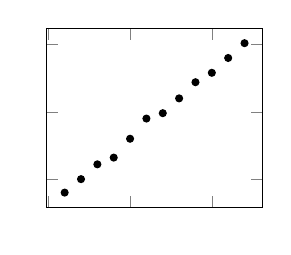
\begin{tikzpicture}
    \begin{axis}[%
        scale=0.4,
        yticklabels={,,},
        xticklabels={,,},
        scatter/classes={a={mark=*,draw=black,mark size=1.25pt,}}
    ]
        \addplot[scatter,only marks,scatter src=explicit symbolic]%
            table[meta=label
        ] 
        {
            x y label
            1 4 a
            2 5 a
            3 6.1 a
            4 6.6 a
            5 8 a
            6 9.5 a
            7 9.9 a
            8 11 a
            9 12.2 a
            10 12.9 a
            11 14 a
            12 15.1 a
        };
    \end{axis}
\end{tikzpicture}\\
{\footnotesize\itshape strong positive correlation}\\
\end{tabular}
\hfill
\begin{tabular}{c}
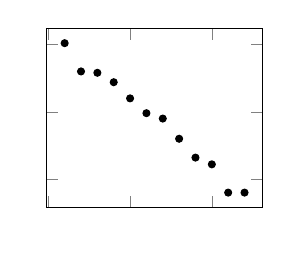
\begin{tikzpicture}
    \begin{axis}[%
        scale=0.4,
        yticklabels={,,},
        xticklabels={,,},
        scatter/classes={a={mark=*,draw=black,mark size=1.25pt,}}
    ]
        \addplot[scatter,only marks,scatter src=explicit symbolic]%
            table[meta=label
        ] 
        {
            x y label
            12 4 a
            11 4 a
            10 6.1 a
            9 6.6 a
            8 8 a
            7 9.5 a
            6 9.9 a
            5 11 a
            4 12.2 a
            3 12.9 a
            2 13 a
            1 15.1 a
        };
    \end{axis}
\end{tikzpicture}\\
{\footnotesize\itshape strong negative correlation}\\
\end{tabular}
\hfill
\begin{tabular}{c}
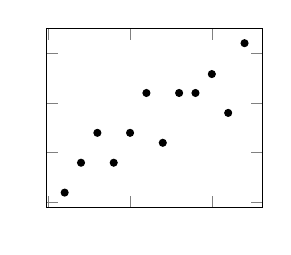
\begin{tikzpicture}
    \begin{axis}[%
        scale=0.4,
        yticklabels={,,},
        xticklabels={,,},
        scatter/classes={a={mark=*,draw=black,mark size=1.25pt,}}
    ]
        \addplot[scatter,only marks,scatter src=explicit symbolic]%
            table[meta=label
        ] 
        {
            x y label
            1 1 a
            2 4 a
            3 7 a
            4 4 a
            5 7 a
            6 11 a
            7 6 a
            8 11 a
            9 11 a
            10 12.9 a
            11 9 a
            12 16 a
        };
    \end{axis}
\end{tikzpicture}\\
{\footnotesize\itshape weak positive correlation}\\
\end{tabular}
\hfill
\begin{tabular}{c}
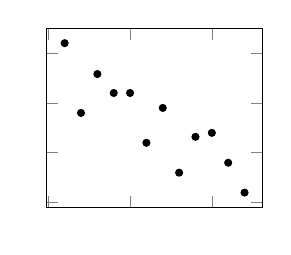
\begin{tikzpicture}
    \begin{axis}[%
        scale=0.4,
        yticklabels={,,},
        xticklabels={,,},
        scatter/classes={a={mark=*,draw=black,mark size=1.25pt,}}
    ]
        \addplot[scatter,only marks,scatter src=explicit symbolic]%
            table[meta=label
        ] 
        {
            x y label
            12 1 a
            11 4 a
            10 7 a
            9 6.6 a
            8 3 a
            7 9.5 a
            6 6 a
            5 11 a
            4 11 a
            3 12.9 a
            2 9 a
            1 16 a
        };
    \end{axis}
\end{tikzpicture}\\
{\footnotesize\itshape weak negative correlation}\\
\end{tabular}
\hfill
}

\begin{center}
\renewcommand{\arraystretch}{0.5}
\begin{tabular}{c}
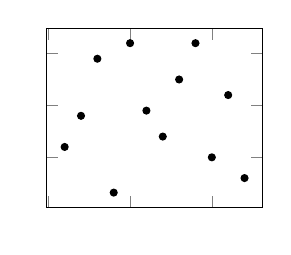
\begin{tikzpicture}
    \begin{axis}[%
        scale=0.4,
        yticklabels={,,},
        xticklabels={,,},
        scatter/classes={a={mark=*,draw=black,mark size=1.25pt,}}
    ]
        \addplot[scatter,only marks,scatter src=explicit symbolic]%
            table[meta=label
        ] 
        {
            x y label
            1 11 a
            2 14 a
            3 19.5 a
            4 6.6 a
            5 21 a
            6 14.5 a
            7 12 a
            8 17.5 a
            9 21 a
            10 10 a
            11 16 a
            12 8 a
        };
    \end{axis}
\end{tikzpicture}\\
{\footnotesize\itshape no}\\{\footnotesize\itshape correlation}\\
\end{tabular}
\end{center}


\myProblemsWithContent[%
    What kind of correlation do you see in these scatterplots?
    \vspace{-1\onelineskip}
    \begin{itemize}[nosep]
        \item strong? weak? none? 
        \item positive? negative?
    \end{itemize}
    ]
{
    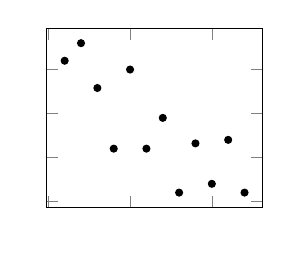
\begin{tikzpicture}
        \begin{axis}[%
            scale=0.4,
            yticklabels={,,},
            xticklabels={,,},
            scatter/classes={a={mark=*,draw=black,mark size=1.25pt,}}
        ]
            \addplot[scatter,only marks,scatter src=explicit symbolic]%
                table[meta=label,row sep=\\] 
            {
                x y label\\
                12 1 a\\
                11 7 a\\
                10 2 a\\
                9 6.6 a\\
                8 1 a\\
                7 9.5 a\\
                6 6 a\\
                5 15 a\\
                4 6 a\\
                3 12.9 a\\
                2 18 a\\
                1 16 a\\
            };
        \end{axis}
    \end{tikzpicture}    
}
{
    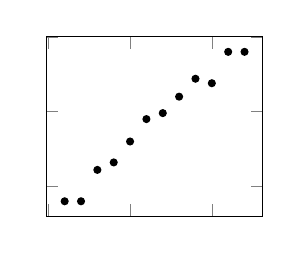
\begin{tikzpicture}
        \begin{axis}[%
            scale=0.4,
            yticklabels={,,},
            xticklabels={,,},
            scatter/classes={a={mark=*,draw=black,mark size=1.25pt,}}
        ]
            \addplot[scatter,only marks,scatter src=explicit symbolic]%
                table[meta=label,row sep=\\] 
            {
                x y label\\
                1 4 a\\
                2 4 a\\
                3 6.1 a\\
                4 6.6 a\\
                5 8 a\\
                6 9.5 a\\
                7 9.9 a\\
                8 11 a\\
                9 12.2 a\\
                10 11.9 a\\
                11 14 a\\
                12 14 a\\
            };
        \end{axis}
    \end{tikzpicture}
}
